\onecolumn 
\section{Anexos}

\begin{figure}[htbp]
    \centering
    \begin{subfigure}[b]{0.48\textwidth}
        \centering
        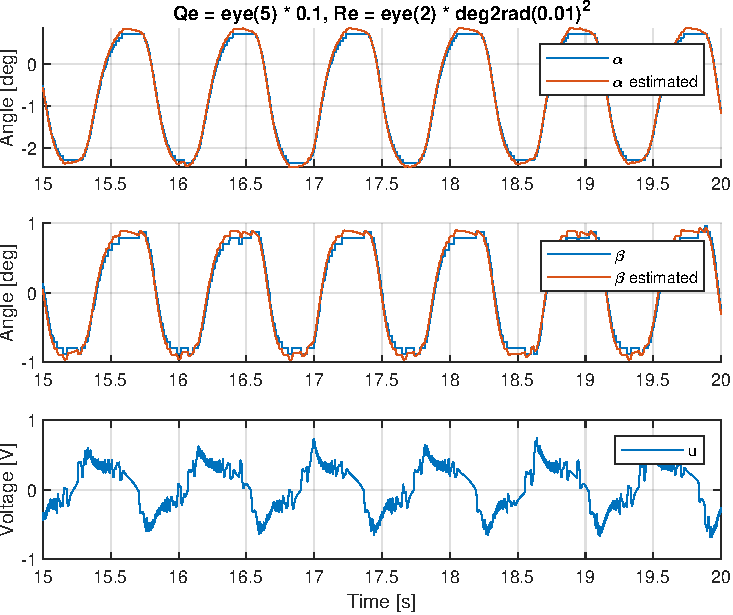
\includegraphics[width=\textwidth]{Body/Images/qe0_1.pdf}
        \caption{$\alpha$ and $\beta$ estimates compared to measurements.}
        \label{fig:qe0_1}
    \end{subfigure}
    \hfill
    \begin{subfigure}[b]{0.48\textwidth}
        \centering
        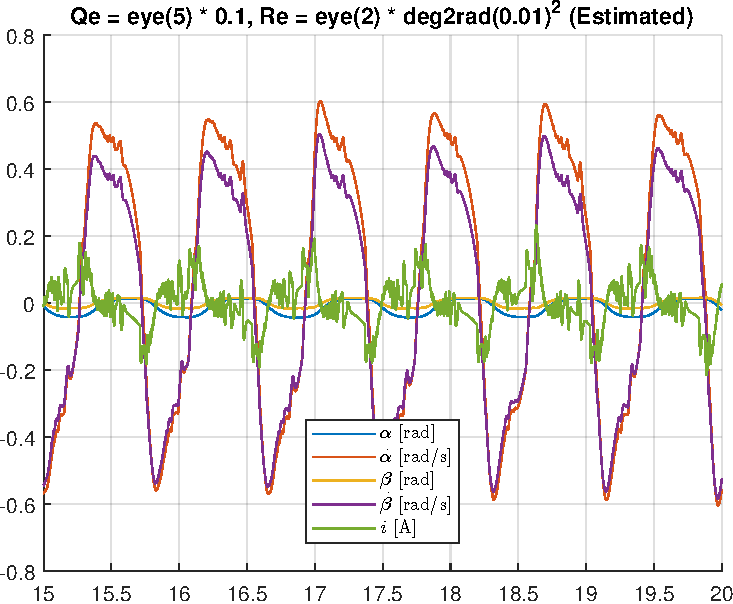
\includegraphics[width=\textwidth]{Body/Images/qe0_1_estimated.pdf}
        \caption{Unmeasured states $\hat{\dot{\alpha}}$, $\hat{\dot{\beta}}$, and $\hat{i}$ and measured states.}
        \label{fig:qe0_1_estimated}
    \end{subfigure}
    \caption{Experimental results of the LQE validation for $Q_e = 0.1 \cdot I_5$.}
    \label{fig:lqe_plots_qe0_1}
\end{figure}

\begin{figure}[htbp]
    \centering
    \begin{subfigure}[b]{0.48\textwidth}
        \centering
        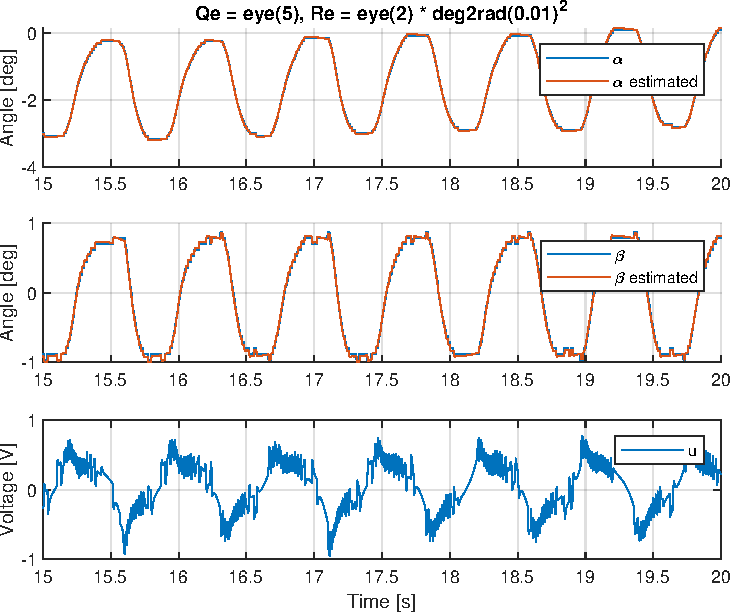
\includegraphics[width=\textwidth]{Body/Images/qe1.pdf}
        \caption{$\alpha$ and $\beta$ estimates compared to measurements.}
        \label{fig:qe1}
    \end{subfigure}
    \hfill
    \begin{subfigure}[b]{0.48\textwidth}
        \centering
        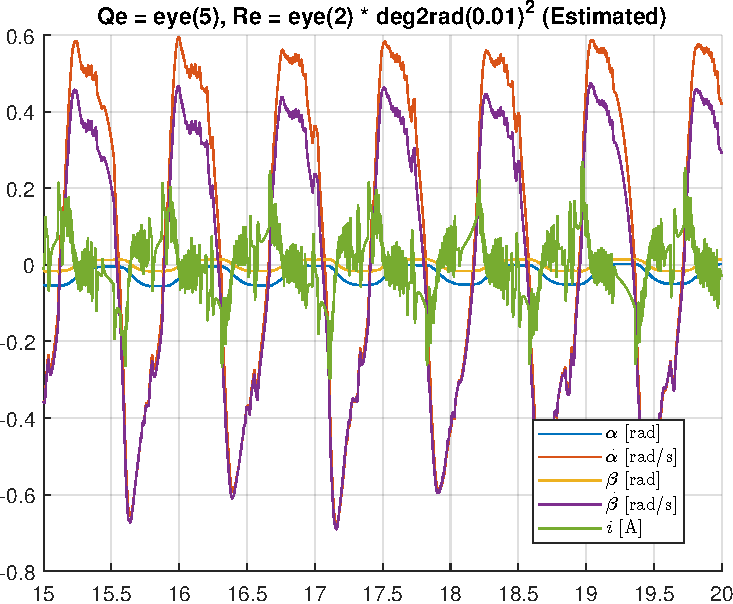
\includegraphics[width=\textwidth]{Body/Images/qe1_estimated.pdf}
        \caption{Unmeasured states $\hat{\dot{\alpha}}$, $\hat{\dot{\beta}}$, and $\hat{i}$ and measured states.}
        \label{fig:qe1_estimated}
    \end{subfigure}
    \caption{Experimental results of the LQE validation for $Q_e = 1 \cdot I_5$.}
    \label{fig:lqe_plots_qe1}
\end{figure}

\begin{figure}[htbp]
    \centering
    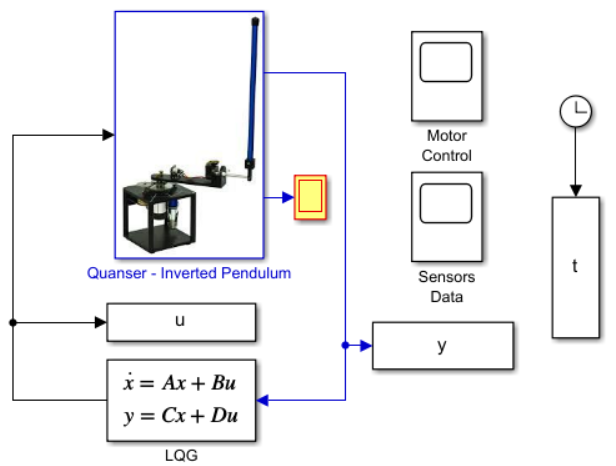
\includegraphics[width=0.8\textwidth]{Body/Images/LQG.png}
    \caption{Simulink implementation of the complete LQG architecture for hardware validation.}
    \label{fig:lqg}
\end{figure}

\begin{figure}[htbp]
    \centering
    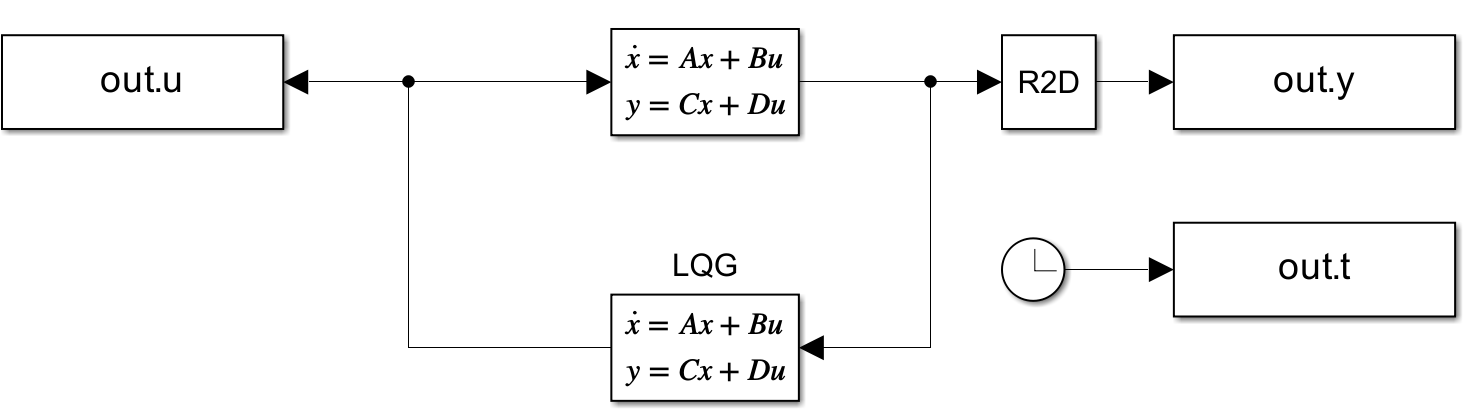
\includegraphics[width=0.8\textwidth]{Body/Images/q11.png}
    \caption{Simulink implementation of the complete LQG architecture for simulation validation.}
    \label{fig:q11}
\end{figure}

\begin{figure}[htbp]
    \centering
    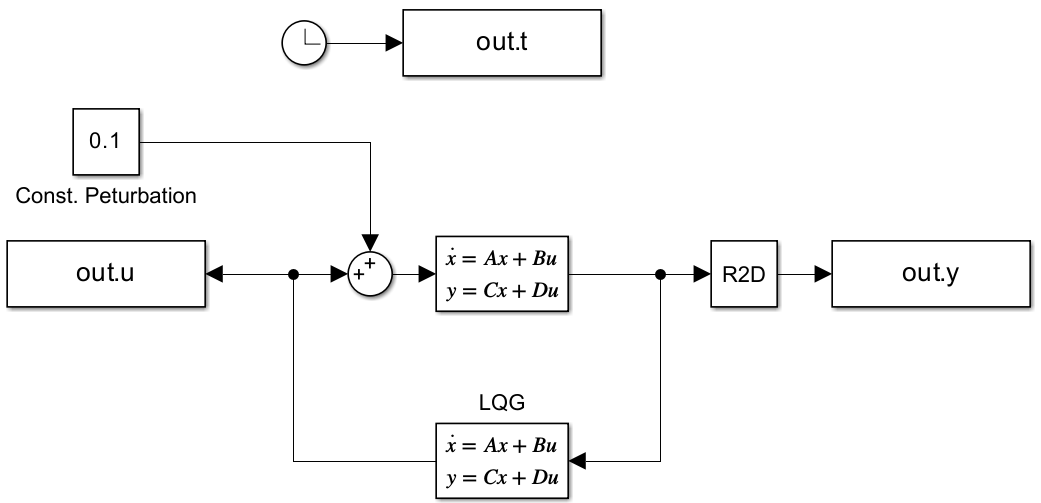
\includegraphics[width=0.8\textwidth]{Body/Images/q11_1.png}
    \caption{Simulink implementation of the complete LQG architecture with a constant perturbation for simulation validation.}
    \label{fig:q11_1}
\end{figure}